
\documentclass[conference]{IEEEtran}

\ifCLASSINFOpdf
 
\else

\fi

\hyphenation{op-tical net-works semi-conduc-tor}

\usepackage{graphicx}
\usepackage{tabularx}
\begin{document}

\title{An Online Interactive Whiteboard \\for Military Applications: a conceptual design}


% author names and affiliations
% use a multiple column layout for up to three different
% affiliations
\author{
\IEEEauthorblockN{Pakamaj Wongsai, Wichai Pawgasame}
\IEEEauthorblockA{Department of Research and Development\\
Defence Technology Institute, Ministry of Defence\\Nonthaburi, Thailand\\
Email: pakamaj.w@dti.or.th}
}





% use for special paper notices
%\IEEEspecialpapernotice{(Invited Paper)}




% make the title area
\maketitle


\begin{abstract}
An Interactive Whiteboard (Virtual Whiteboard) may refer to a device or a computer program providing interactive displays. 
%%
This interactive whiteboard along with online system can provide efficient interactive long-distance conferencing, training, or educating systems. 
%%
These systems have been extensively used in classrooms and meeting rooms. 
%%
In fact, the use of online interactive whiteboard can be applied for the military as a distributed mission planning system. 
%%
An information can be shared locally through LAN or globally through Internet. 
%%
This concept is relatively challenged due to the limitations of military networks in terms of security, frequency, bandwidth, and computational power of the equipment. 
%%
This paper introduces a novel online interactive whiteboard design framework that specifically aim at the military application.      
\end{abstract}

\IEEEpeerreviewmaketitle


%%%%%%%%%%%%%%%%%%%%%%%%%%%%%%%%%%%%%% 
\section{Introduction}
%%%%%%%%%%%%%%%%%%%%%%%%%%%%%%%%%%%%%% 

A military operation involves common three-step process; planning, preparing, and execute. 
%%
To accomplish the mission, a commander and his supporting staffs must drive the operation processes through understanding, visualizing, describing, directing, and assessing \cite{AA}. 
%%
A mission planner is a tool to help a commander and staffs utilizing the those operation processes. 
%%
The use of online interactive whiteboard as mission planning tool can make operation be more effective. 
%%
An online interactive whiteboard is a device or a program that allows participants from different locations to share the same whiteboard screen. 
%%
The participants can change content of the screen and in addition the updated screen can be distributed among the participant in real-time.  
%% 
More over, participants can create common understanding of the operation using online interactive whiteboard. 
%%
An online interactive whiteboard provides visualization for situation understanding and determining desire goal. 
%%
An operation can be described to all participants to shared understanding and purpose using the online interactive whiteboard. 
%%
A commander may use an online interactive whiteboard to direct the mission by establishing an intent, setting objectives, and issuing clear tasks to subordinate units. 
%%
An online interactive whiteboard provides an overview of the plan to ease the assessment process of the plan. 
%%
The participants should be able to join a discussion, leave a discussion, and add information to the whiteboard while always having an up-to-date image of the current whiteboard. 
%%
An online interactive whiteboard is a network application or device, where the information is exchanged globally via Internet or locally LAN. 
%%
The online interactive whiteboard systems have been extensively used in the classrooms and civilian meeting rooms depending on public networks. 
%%
The military application operates in different networks designed specifically for military operation. 
%%
Due to limitation of military networks in terms of security, frequency, bandwidth, and computational power of the equipment, the design of an online interactive whiteboard require a novel approach.
%% 
This paper introduces a novel online interactive whiteboard design framework that specifically aim at the military application over Internet. 
%%
The organization of this paper is as followings. Section II presents background concept and theory behind an online interactive whiteboard. Section III proposes an overview of the system. Section IV discusses design consideration. Section V presents the specification of the design framework in application layer. Finally, the summary of the work is given in Section VI.


%%%%%%%%%%%%%%%%%%%%%%%%%%%%%%%%%%%%%% 
\section{Background}
%%%%%%%%%%%%%%%%%%%%%%%%%%%%%%%%%%%%%% 

\subsection{Mission Planner}
An mission planning is an art that requires an in-depth understanding of numerous critical elements or factors that may impact the mission and an assessment of how those elements or factors can be either negated, overcome or exploited to give the advantage it requires in the execution of the mission. 
%%
The role of on-going real-time intelligence plays a crucial role in the planning of the mission. 
%%
It is also this intelligence that will ultimately determine the mission-profile. 
%%
The mission-profile, in turn, will determine the amount of manpower, weapons, ammunition, the phases of war, tactics, etc \cite{AB}.
%%
In fact , planning is considered a vital component for success of any mission. 
%%
A Team leader must be allowed to display flexibility within the overall plan and, in turn, must develop their own plans at their level. 
%%
The ultimate aim of planning is to ensure that the correct men, correctly equipped, are at the right time and place to achieve the mission. 
%%
This requires constant coordination between the various elements that will partake in the execution of the plan. 
%%
With this concept, the casualties can be reduced. 

%%%%%%%%%%%%%%%%%%%%%%%%%%%%%%%%%%%%%% 
\subsection{Interactive Whiteboard}

An interactive whiteboard is a device or a computer program providing interactive display.
%% 
Typically an interactive whiteboard contains a sensor device that capture the movement on the whiteboard’s screen. 
%%
The captured movements are then processed by the computer, which can be resided in whiteboard or as separated device. 
%%
Consequently, the processed movement is visualized in screen and can interact with each object on screen. 
%%
The networking of interactive whiteboard can provide corporative interaction between the presenters and audiences. 
%%
This interactive whiteboard is a technology that can assist teachers, trainers, or meeting leaders to efficiently interact with the audiences. 
%%
In some classrooms, interactive whiteboards have been replaced traditional whiteboard. 
%%
From this point of view, the interactive whiteboard can be applied to the military's mission planning for real-time mission planning that can be distributed to all involved units.

\begin{figure*}[t]
\begin{center}
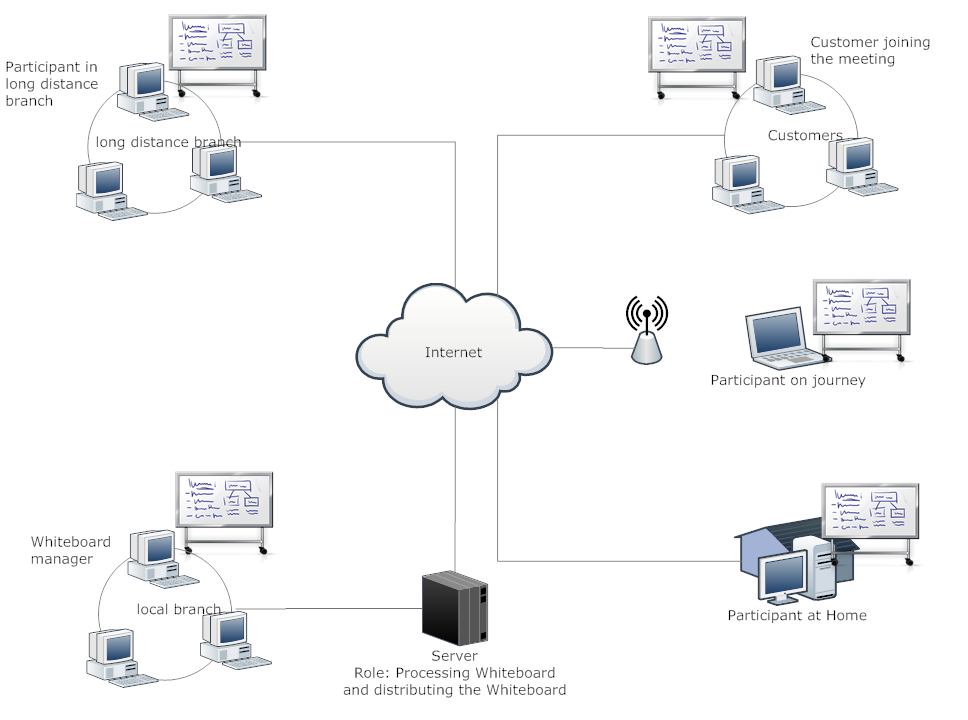
\includegraphics[width=0.7\textwidth]{iw_system_overview.png}
\caption{Online Interactive Whiteboard System for military application}
\label{fig:1}
\end{center}
\end{figure*}

%%%%%%%%%%%%%%%%%%%%%%%%%%%%%%%%%%%%%% 
\subsection{TCP/IP Model}

A TCP/IP model or Internet model is a networking model and communications protocols that commonly used on the Internet. 
%%
Normally, TCP/IP model specifies how data should be transmitted and received on the internet. The model is organised into four abstraction layers, in which each layer contains related protocols according to involved networking functionalities \cite{RFC1122, RFC1123}.
%%
The layers of the TCP/IP model are application layer, transport layer, internet layer, and link layer. 
%%
The types of services performed and protocols used at each layer within the TCP/IP model are described in more detail in Table \ref{tab:1}. 
%%
Application layer provides process-to-process application data exchange. 
%%
The transport layer handles host-to-host communication. Internet layer establishes internetworking between networks. 
%%
The link layer defines how data is physically sent and received over single link. 
%%
This paper proposes the design framework for an online interactive whiteboard that specifies suitable protocols for each layer in TCP/IP model.

\begin{table}[h]
  \renewcommand{\arraystretch}{2}
  \renewcommand{\tabcolsep}{2mm}
 
  \begin{tabularx}{0.5\textwidth}{|p{1.5cm}|p{4.3cm}|p{2cm}|}
    \hline
    \multicolumn{1}{|c|}{\textbf{Layer}} &  
    \multicolumn{1}{c|}{\textbf{Description}} &
    \multicolumn{1}{c|}{\textbf{Protocols}} \\ \hline
    \textbf{Application} &  Defines TCP/IP application protocols and how host programs interface with transport layer services to use the network. & HTTP, Telnet, FTP, TFTP, other application protocols \\ \hline 
    \textbf{Transport} &  Provides communication session management between host computers. Defines the level of service and status of the connection used when transporting data. & TCP, UDP, RTP \\ \hline 
     \textbf{Internet} &  Packages data into IP datagrams, which contain source and destination address information that is used to forward the datagrams between hosts and across networks. Performs routing of IP datagrams. & IP, ICMP, ARP, RARP \\ \hline 
     \textbf{Link} &  Specifies details of how data is physically sent through the network, including how bits are electrically signaled by hardware devices that interface directly with a network medium, such as coaxial cable, optical fiber, or twisted-pair copper wire. & Ethernet, Token Ring, FDDI, X.25, Frame Relay, RS-232, v.35 \\ \hline 
  \end{tabularx}
  \space
  \caption{Services and Protocols of TCP/IP Model}
  \label{tab:1}
\end{table}

%%%%%%%%%%%%%%%%%%%%%%%%%%%%%%%%%%%%%%
\section{System Overview}
%%%%%%%%%%%%%%%%%%%%%%%%%%%%%%%%%%%%%%

The online interactive whiteboard is the electronic whiteboard with the client-server program, where the information drawn on whiteboard is exchanged through internet or LAN in real-time. 
%%
There are two parts of application: client application and server application. 
%%
The designed application works in client-server manner.  
%%
Figure \ref{fig:1} illustrates the structure of system.

%%%%%%%%%%%%%%%%%%%%%%%%%%%%%%%%%%%%%%  
\subsection{Server}

The server is responsible for the processing request and distributing the up-to-date whiteboard screen in real-time. 
%%
The server is responsible for initializing new whiteboard session when there is a request and handles invitation, joining and leaving requests to the whiteboard. 
%%
The server also contains database storing information about system members and whiteboard session history. 
%%
It also handles the authentication to the system. 
%%
The server should be able to handle multiple requests and distribute information in shortest time, so that the system meet real-time need in the military operation.

%%%%%%%%%%%%%%%%%%%%%%%%%%%%%%%%%%%%%%
\subsection{Client}

In the system, there are two roles of clients: whiteboard manager and participant.  
%%
Firstly, the whiteboard manager is the member who requests for the new whiteboard allocation. 
%%
The participant can join the whiteboard by an invitation from whiteboard manager or authorized request for joining the whiteboard. 

%%%%%%%%%%%%%%%%%%%%%%%%%%%%%%%%%%%%%%
\subsection{Network}

The proposed system is operated in IP-based network environment. 
%%
This system should be able to work with existing Internet network without installation of new network hardware.  
%%
The server can be placed inside the headquarter or the center of command and control unit. 
%%
Each client can communicate through existing military's Internet connections. 

%%%%%%%%%%%%%%%%%%%%%%%%%%%%%%%%%%%%%%
\section{Design Consideration}
%%%%%%%%%%%%%%%%%%%%%%%%%%%%%%%%%%%%%%

\subsection{Data messages}
%%%%%%%%%%%%%%%%%%%%%%%%%%%%%%%%%%%%%%

The virtual whiteboard should be able to present and distribute data on whiteboard to all participants. 
%%
The whiteboard screen on each participant should be updated as fast as real-time. 
%%
All participants will use the same screen configurations such as screen size. 
%%
The screen can be synchronized according to synchronization messages. 
%5
Instead of sending the whole screen as media stream, only stroke data will be sent along with the instruction message at the beginning and the end as illustrated in figure \ref{fig:2}. 
%%
Stroke data is the stream of samples containing position on screen and sequence number. 
%%
Clients use this stroke stream to reconstruct the stroke at its own screen. 

\begin{figure}[h]
\begin{center}
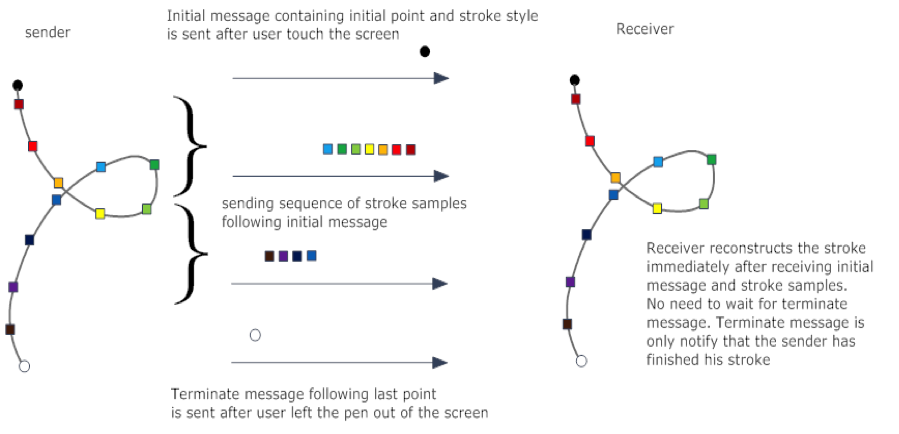
\includegraphics[width=0.5\textwidth]{iw_stroke_transmission.png}
\caption{Stroke transmission scheme}
\label{fig:2}
\end
{center}
\end{figure}

In addition to whiteboard synchronization message, there is a system authorization message used to establish and terminate connection between single client and the server, whiteboard initialization message that is responsible for initiating whiteboard space and session to be used among specific group, invitation message that takes care of sending whiteboard invitation to connected user, and joining and leaving message that handles joining request to existing whiteboard session.

%%%%%%%%%%%%%%%%%%%%%%%%%%%%%%%%%%%%%%
\subsection{Security}

There might be some information on whiteboard that should be kept secret among group. 
%%
Therefore, data security is definitely required. 
%%
One solution is to use data encryption.
%%
Basically, the encoding information is related to mathematical methods to protect the raw data or text that needed to sent to the recipient. 
%%
Raw data are turned into text data or other forms of understanding that cannot read by anyone who does not have the key for reviewing that information. 
%%
The process of transforming the initial information is called \emp{Encrypted data or data Encryption}. 
%%
On the other hand, the conversion process that transforms unreadable information back to the original text is called the decoding information or decryption. There are 2 main types of encrypt data algorithms

%%%%%%%%%%%%%%%%%%%%%%%%%%%%%%%%%%%%%%
\subsection{Transport Layer}
Transport Layer performs similar functions to the Network layer in controlling the quality of the sending and receiving data. 
%%
If there is an error occurring in the network or network failure, the transport layer will look for the other route that leads to the destination. 
%%
It will also store the sent data until the new network connection is established. 
%%
In this paper, Stream Control Transport Protocol (SCTP) is chosen due to many advantages comparing to other protocols as listed in table . 
%%
One of the key advantage is the supporting of multi-streaming. 

\begin{table}[h]
  \renewcommand{\arraystretch}{2}
  \renewcommand{\tabcolsep}{2mm}
  \centering
  \begin{tabularx}{0.5\textwidth}{|p{4.4cm}|p{1cm}|p{1cm}|p{1cm}|}
    \hline
    \multicolumn{1}{|c|}{\textbf{Services/Features}} &  
    \multicolumn{1}{c|}{\textbf{SCTP}} &
    \multicolumn{1}{c|}{\textbf{TCP}} &
    \multicolumn{1}{c|}{\textbf{UDP}} \\ \hline
    Full-duplex &  yes & yes & yes \\ \hline 
    Connection-oriented & yes & yes & no \\ \hline 
    Reliable data transfer & yes & yes & no \\ \hline 
    Ordered data delivery & yes & yes & no \\ \hline 
    Flow and congestion control & yes & yes & no \\ \hline
    Data fragmentation & yes & yes & no \\ \hline
    Multi-streaming & yes & no & no \\ \hline
    Multi-homing & yes & no & no \\ \hline
    SYN flooding attack protection & yes & no & n/a  \\ \hline
  \end{tabularx}
  \space
  \caption{Services and Protocols of TCP/IP Model}
  \label{tab:1}
\end{table}

SCTP operation is similar to TCP, but the characteristic of the data is similar to the one in UDP. 
%%
SCTP is the message-oriented protocol, while TCP is the stream-oriented protocol. 
%%
It supports many mandatory features including multi-homing, multi-streaming, three delivery modes (ordered delivery, unordered delivery, and partially ordered), selective acknowledgment support (SACK), heartbeat keep-alive mechanism and DoS protection. 
%%
The data in SCTP, or SCTP packet, is identified by IP address. 
%%
Each SCTP packet consists of header and chucks, and is divided into many small parts. 

%%%%%%%%%%%%%%%%%%%%%%%%%%%%%%%%%%%%%%
\subsection{Internet Layer}

The existing Internet connection will be used as the backbone network. 
%%
The application should support both IPv4 and IPv6. 
%%
In fact, IPv6 is already backward compatible with IPv4, provided that special techniques are used.
%%
To support IPv4/IPv6 compatibility, a scheme was developed to allow IPv4 addresses to be embedded within the IPv6 address structure. 
%%
This method takes regular IPv4 addresses and puts them in a special IPv6 format so they are recognized as being IPv4 addresses by certain IPv6 devices.
%%
Since the IPv6 address space is so much bigger than that of IPv4, embedding the latter within the former is easy; it's like tucking a compact sedan into the hold of a cargo ship. 
%%
The embedding address space is part of the reserved address block whose addresses begin with eight zero bits, but only a relatively small part of it.
%%
Two different embedding formats are used. 
%%
Both have zeros for the first 80 bits of the address, and put the embedded IPv4 address into the last 32 bits of the IPv6 address format. 
%%
They differ on the value of the 16 remaining bits in between (bits 81 to 96, counting from the left). 
%%
These embedding techniques are already implemented in most existing network devices and operating system. Therefore, there should not be any problem whether IPv4 or IPv6 is used.

%%%%%%%%%%%%%%%%%%%%%%%%%%%%%%%%%%%%%%
\subsection{Input and Output Device}

A touch screen can be used as an interface device for input and output data. 
%%
It is basically the device that can be use as both the input, as mouse or keyboard, and output, as the normal display monitor. 
%%
The main component of the touch screen is the contact sensor under the control board which will analyze the signal received from the sensor for the exact coordination of the contact place. 

%%%%%%%%%%%%%%%%%%%%%%%%%%%%%%%%%%%%%%
\section{Specification of Online Interactive Whiteboard Application}
%%%%%%%%%%%%%%%%%%%%%%%%%%%%%%%%%%%%%%

With the design consideration proposed in previous section, figure \ref{fig:4} summarizes the protocol applied to each layer of TCP/IP model. 
%%
This section gives detailed specification of application protocol for the online interactive whiteboard system.
 
 \begin{figure}[h]
\begin{center}
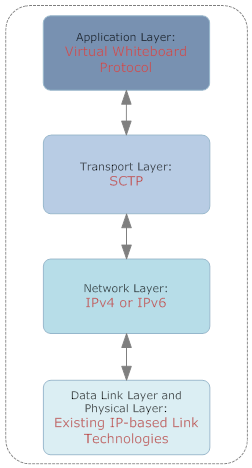
\includegraphics[width=0.3\textwidth]{iw_tcpip.png}
\caption{TCP/IP Model of the online interactive whiteboard}
\label{fig:3}
\end{center}
\end{figure}
 \begin{figure*}[t]
\begin{center}
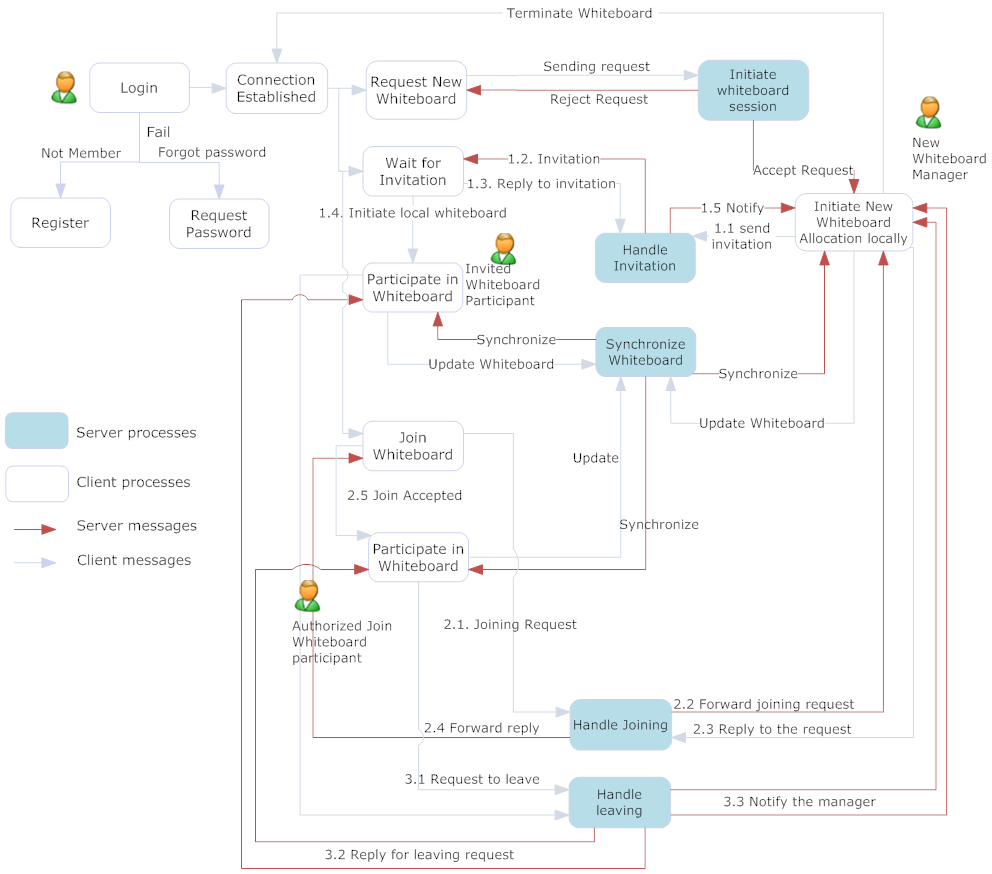
\includegraphics[width=0.8\textwidth]{process}
\caption{The online interactive whiteboard process}
\label{fig:4}
\end{center}
\end{figure*}

%%%%%%%%%%%%%%%%%%%%%%%%%%%%%%%%%%%%%%
\subsection{Application Roles}

Application can take on three roles: The server role operates on server application, the manager and participant roles operate on client application

%%%%%%%%%%%%%%%%%%%%%%%%%%%%%%%%%%%%%%
\subsubsection{Server Role}

The server is responsible for the processing of whiteboard and distributing the up-to-date whiteboard in real-time. 
%%
The server is responsible for initializing new whiteboard session when there is a request and handles invitation, joining and leaving requests to the whiteboard. 
%%
The server receives the new whiteboard details from participants and synchronizing new details to all participants. 
%%
All participants should be synchronized to the same up-to-date whiteboard. 
%%
The server does not actually distribute the whiteboard screen, but it distributes the action done by participant. 
%%
The clients received this distributed information can update their own whiteboard accordingly. 
%%
The server also contains database storing information about system members and whiteboard session history. 
%%
It also handles the authentication to the system. 
%%
The server should be able to handle multiple requests and distribute information in shortest time, so that the system is working as close as the real-time.

%%%%%%%%%%%%%%%%%%%%%%%%%%%%%%%%%%%%%%
\subsubsection{Manager Role}

A whiteboard manager is the member who requests for the new whiteboard allocation.
%%
This manager can invite other members to participate in whiteboard. 
%%
He can authorize other members to join in the whiteboard. 
%%
Consequently, a whiteboard manager is the only one who can end the whiteboard session. 
%%
The manager is eligible to update content of whiteboard during whiteboard session at anytime

%%%%%%%%%%%%%%%%%%%%%%%%%%%%%%%%%%%%%%
\subsubsection{Participant Role}
A participant can join the whiteboard by invitation from whiteboard manager or authorized request for joining the whiteboard. 
%%
In addition, the participants can leave the whiteboard at anytime during whiteboard session and they can join again with authorization from the whiteboard manager. 
%%
Finally, the participants are eligible to update content of whiteboard just like whiteboard manager.

%%%%%%%%%%%%%%%%%%%%%%%%%%%%%%%%%%%%%%
\subsection{Application Process}

The server application should always be running and ready to serve client application.
%%
When the client application is started, it create socket for communication with the server. 
%%
The communication with system has not been established yet.  
%%
Client needs to login to establish a connection by sending authorization request message to the server. 
%%
When the login information is authorized by the server, the server registers the client along with its socket address and sends the acknowledgment message back to client. 
%%
A client is now ready to send or receive message from server. 
%%
Consequently, a client socket stays open until client logs out.
%%
After logging in to the system, clients are able to create whiteboard. 
%%
The client, who creates whiteboard, becomes the whiteboard manager of that whiteboard session. 
%%
The process of creating whiteboard is initiated by the client side. 
%%
The client sends a request to initiate whiteboard. 
%%
Upon receiving the request, the server checks whether or not this client involves in any other whiteboard session. 
%%
In the case of involvement, the request is rejected. 
%%
If not, the request is accepted and the server allocates database space for recording whiteboard history. 
%%
This space contains information about whiteboard session ID, manager ID, participant ID, and synchronization history. 
%%
This feature enable playback of the old whiteboard sessions. 
%%
After allocating space for whiteboard session, the server sends acknowledgment to the client. 
%%
Then the client changes its role to whiteboard manager.
%%
A whiteboard manager has an ability to invite other clients to the whiteboard session. 
%%
The clients that are eligible for invitation must have already been authorized by the server through the login process and must not have involved in any whiteboard session.
%%
The available client lists are distributed to the manager by the server. 
%%
The invitation process starts when manager sends the invitation message to one or more clients. It is not peer-to-peer communication. 
%%
The invitation message is received by the server first. 
%%
The server searches for socket address specific for each destination. 
%%
Then, it forwards the invitation message to all destinations. 
%%
Upon receiving the invitation message, the clients have an option to accept or reject invitation. 
%%
The reply message is sent back to the server. 
%%
The server registers the client to whiteboard session and sends notification message to the manager, if the answer is yes. 
%%
If the answer is no, the server just sends notification message to the manager. 
%%
The clients accepting invitation becomes participants in whiteboard session.
%%
A whiteboard session is not blinded from other clients. 
%%
Clients in the system can see a list of whiteboard session, but cannot see what is inside. 
%%
The clients are able to join any whiteboard session with permission from the corresponding whiteboard manager. 
%%
A client currently logged into the system can send the joining request to the manager. 
%%
Just like invitation message, joining message is not peer-to-peer communication. 
%%
The message is sent to server, then server forward message to the manager. 
%%
After receiving joining request, the manager decides on accepting or rejecting the request. 
%%
The reply message is sent out to server. 
%%
The server checks whether the answer is yes or no. 
%%
If the answer is yes, then the server registers requesting client to the whiteboard session, and notifies both new participant and the manager. 
%%
The whiteboard screens on new participants application are synchronized to the up-to-date screen using whiteboard synchronization history stored in the server.
%%
The participants can leave the whiteboard session anytime by sending leaving request to the server. 
%%
A server unregisters participant who is sending leaving request from whiteboard session.
%%
Then, the server sends notify message to both leaving client and manager. 
%%
A leaving client can request joining the whiteboard session again as long as the session still running. 
%%
The leaving clients are not terminated from the system. 
%%
To be terminated from system, client must log out from system. 
%%
If the server crashes, then all client connections are terminated. 
%%
Figure \ref{fig:4} illustrates the overall process of the online interactive whiteboard

What will happen if the client never left the pen out of the screen? 
%%
The stroke samples will be indefinitely long. 
%%
This is a waste because these stroke samples are not useful information. 
%%
To overcome this problem, the client application sets the timer when stroke samples start to be on the same position for many samples. 
%%
When the timer ends and the position does not change, then the terminate message will be sent to end the current stroke. 
%%
With multi-streaming capability of SCTP, multiple strokes can be sent simultaneously.

%%%%%%%%%%%%%%%%%%%%%%%%%%%%%%%%%%%%%%
\section{Summary}
%%%%%%%%%%%%%%%%%%%%%%%%%%%%%%%%%%%%%%
An online interactive whiteboard for military application is based on IP network technologies. 
%%
The proposed system will be operated in client-server model. 
%%
The SCTP is selected as a transport layer, because it provides many features suitable for multi-stream application. 
%%
The application can provide the information closed to real-time. 
%%
In this paper, the application processes in both client and server have been discussed. 
%%
In addition, data messages and transmission scheme are discussed and presented, which can give enough information for high level programmer for future implementation of the system. 
%%
Other consideration such as security and network difficulties are included as well. 
%%
An online interactive whiteboard will be useful in future military operation where real-time distribution and updating of plan is crucial.

\begin{thebibliography}{1}

  \bibitem{AA} {\em The Operation Process}, Army Doctrine Publication, No. 5-0, Headquarter, Department of the Army, Washington, DC, May 17, 2012. [Online]. Available: Army Knowledge Online.

  \bibitem{AB} {\em The Impotance of Mission Planner}, Jun. 6, 2009. [Online]. Available: http://eebenbarlowsmilitaryandsecurityblog.blogspot.com/2009/06/importance-of-mission-planning.html. [Access: Dec. 20,2014].
  
  \bibitem{RFC1122} RFC 1122,{\em Requirements for Internet Hosts-Communication Layers,} R. Braden (ed.), October 1989.
  
  \bibitem{RFC1123} RFC 1123,{\em Requirements for Application and Support,} R. Braden (ed.), October 1989.
  
  
\end{thebibliography}


\end{document}


